\section[Mean-feild]{Mean-field result of the two-channel models}

\frame{
\frametitle{Extremely narrow resonance}
The coupling between two channels is assumed to be extremely weak. $\delta_{c}\to0$. Two channels share the same chemical potentials. 
\begin{figure}[hhtb]
	\centering
	         \subfloat[$E_{F}<\tilde\delta$]{\label{fig:narrowFR:aboveSea}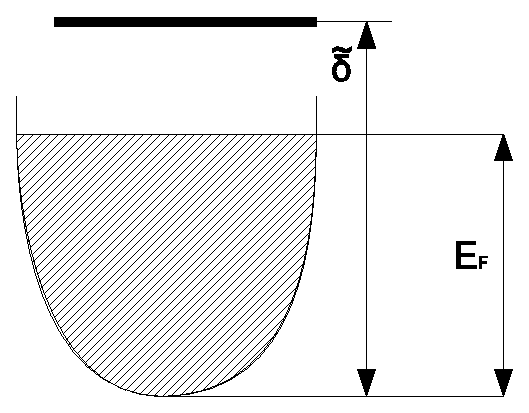
\includegraphics[width=.2\textwidth]{narrowFRabove.eps}}\quad
		\subfloat[$0<\tilde\delta<E_{F}$]{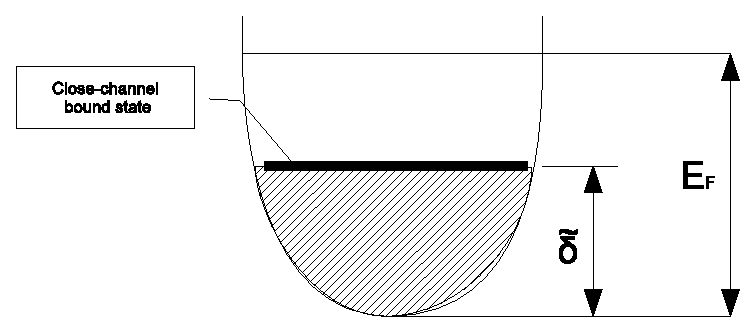
\includegraphics[width=.30\textwidth]{narrowFRin.eps}\label{fig:narrowFR:inSea}}\quad
		\subfloat[$\tilde\delta<0$]{\label{fig:narrowFR:belowSea}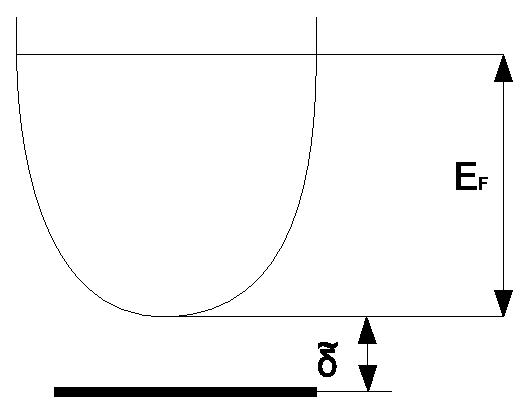
\includegraphics[width=.20\textwidth]{narrowFRbelow.eps}}
	\caption{Extremely narrow resonance\label{fig:narrowFR}}
	\small{The shaded area is occupied by atoms. }
	%\parbox{0.7\textwidth}{\small{  In Fig. \subref{fig:narrowFR:inSea} chemical potential would be close to the closed-channel bound state level (besides small shift due to the open-channel intra-channel coupling) and the ``Fermi sea'' above is empty. }}
\end{figure}
}



\frame{
\frametitle{Model setup}


The finite-temperature action is 
\begin{equation}
\begin{split}\label{eq:pathInt2:actionFermi}
&S(\bar\psi,\psi)=\int^{\beta}_{0}d\tau\int{d^{d}r}\\
&\Big[\sum_{j}\bar\psi_{j}(\partial_\tau-\nth{2m}\nabla^{2}-\mu+\eta_{j})\psi_{j}
-(\bar\psi\bar\psi)\tilde{U}(\psi\psi)\Big]
\end{split}
\end{equation}
$\eta_{j}$ is the Zeeman energy of the hyperfine species j. Two channels are expressed as a 2-component vector
\begin{equation*}
(\bar\psi\bar\psi)=\mtrx{\bar\psi_{a}\bar\psi_{b}&\bar\psi_{a}\bar\psi_{c}}
\qquad(\psi\psi)=\mtrx{\psi_{b}\psi_{a}\\\psi_{c}\psi_{a}}
\end{equation*}
We have \myemph{contact} interaction 
\begin{equation}
\tilde{U}\equiv{}\mtrx{U&Y\\Y^{*}&V}
\end{equation}



}

\frame{
\frametitle{Hubbard-Stratonovich transformation}
Introduce a two-component auxiliary field
\begin{equation*}
\mtrx{\Delta_{1}\\\Delta_{2}}\longrightarrow
	\mtrx{\Delta_{1}\\\Delta_{2}}-
	\mtrx{U&Y\\Y^{*}&V}
	\mtrx{\psi_{b}\psi_{a}\\\psi_{c}\psi_{a}}
\end{equation*}
This coupling has built-in channel mixture. 

\begin{gather*}
\exp[\int{dx}(\bar\psi\bar\psi)\tilde{U}(\psi\psi)]\\
=\int{\bigD(\Delta,\bar\Delta)}\exp\big\{-\int{dx}
	[\Delta^{\dg}\tilde{U}^{-1}\Delta-(\bar\psi\bar\psi)\Delta-\bar\Delta{}(\psi\psi)]\big\}
\end{gather*}
}

\frame{
\frametitle{Hubbard-Stratonovich transformation (2)}
Introduce  a 3-component spinor similar to the Nambu spinor representation in the single-channel superconductivity.  
\begin{equation}
\bar\Psi=\mtrx{\bar\psi_{a}&\psi_{b}&\psi_{c}}\qquad\Psi=\mtrx{\psi_{a}\\\bar\psi_{b}\\\bar\psi_{c}}
\end{equation}
The action can then be rewritten in a more compact form with respect to $\Psi$ and $\bar\Psi$
\begin{equation}\label{eq:pathInt2:actionMixCompact}
S(\bar\Delta,\Delta,\bar\psi_{i},\psi_{i})=\int^{\beta}_{0}d\tau\int{d^{d}r}
	\mbr{\Delta^{\dg}\tilde{U}^{-1}\Delta-\bar\Psi\mathcal{G}^{-1}\Psi}
\end{equation}
It is bilinear of $\Psi$.  We can integrate it out,
\begin{equation}\label{eq:pathInt2:actionD}
S(\bar{\Delta},\Delta)=\int{dx}\br{\bar{\Delta}\tilde{U}^{-1}\Delta-\tr\ln\nG}
\end{equation}

}

\note{\begin{itemize}
\item This is different from the two-component channel-based vector.
\item For b,c, $\bar\psi$ and $\psi$ are reversed, which gives an extra negative sign.
�
\end{itemize}
}

\frame{
\frametitle{Gor'kov Green function}
where 
\begin{equation}
\mathcal{G}^{-1}=
\begin{pmatrix}\label{eq:pathInt2:nGDelta}
[\hat{G}_{0}^{(p)}]^{-1}-\eta_{a}&\Delta_{1}&\Delta_{2}\\
\bar\Delta_{1}&[\hat{G}_{0}^{(h)}]^{-1}+\eta_{b}&0\\
\bar\Delta_{2}&0&[\hat{G}_{0}^{(h)}]^{-1}+\eta_{c}
\end{pmatrix}
\end{equation}
 $[\hat{G}_{0}^{(p)}]^{-1}=-\partial_{\tau}+\nth{2m}\nabla^{2}+\mu$,  $[\hat{G}_{0}^{(h)}]^{-1}=-\partial_{\tau}-\nth{2m}\nabla^{2}-\mu$ 
Decoupled in the momentum-frequency space
\begin{equation*}\label{eq:pathInt2:nGDeltaK}
\mathcal{G}^{-1}=
\begin{pmatrix}
i\omega_{n}-\xi_{k}-\eta_{a}&\Delta_{1}&\Delta_{2}\\
\bar\Delta_{1}&i\omega_{n}+\xi_{k}+\eta_{b}&0\\
\bar\Delta_{2}&0&i\omega_{n}+\xi_{k}+\eta_{c}
\end{pmatrix}
\end{equation*}
$\xi_{k}=\nth{2m}k^{2}-\mu$
}
\frame{
\frametitle{Diagonalization of the Green's function\label{sec:diagonalGreen}}

\begin{equation}\label{eq:pathInt2:nG}
\mathcal{G}^{-1}=i\omega_{n}I-
\begin{pmatrix}
\xi_{k}&-\Delta_{1}&-\Delta_{2}\\
-\bar{\Delta}_{1}&-\xi_{k}&0\\
-\bar{\Delta}_{2}&0&-(\xi_{k}+\eta)
\end{pmatrix}
\end{equation}
\begin{itemize}
\item
Decoupled in the momentum-frequency space
\item Only need to be diagonalized in the $3\times3$ hyperfine-spin space
\end{itemize}
}

\frame{
\frametitle{Diagonalization of the Green's function (2)}
\begin{equation}\label{eq:pathInt2:B}
B_{\omega_{n},\vk}=L_k^{\dg}T_k^{\dg}G_{\omega_{n},\vk}^{-1}T_kL_k
\end{equation} 
\begin{equation}\label{eq:pathInt2:T}
T_k=\mtrx{u_k&v_k&0\\-v_k&u_k&0\\0&0&1}
\end{equation}	
\begin{gather*}
v_{\vk}^{2}\equiv1-u_{\vk}^{2}\equiv\nth{2}\br{1-\frac{\xi_{\vk}}{E_{\vk}}}\qquad
E_{\vk}\equiv(\xi_{\vk}^{2}+\Delta_{1}^{2})^{1/2}
\end{gather*}
$T_{k}$ is enough to diagonalize the $G$ matrix in the broad resonance case. 
}
\frame{
\frametitle{Diagonalization of the Green's function (3)}
For the narrow resonance,
\begin{equation}\label{eq:pathInt2:Bapprox}
B_{\omega_{n},\vk}=i\omega_{n}I-
	\mtrx{E_{1}{}_{\vk}&0&0\\0&-E_{2}{}_{\vk}&0\\0&0&-E_{3}{}_{\vk}}
%	&\approx{}i\omega_{n}I-
%	\mtrx{E_{\vk}+{}u_{\vk}^{2}\zeta&0&0\\
%	0&-\br{E_{\vk}-{}v_{\vk}^{2}\zeta}&0\\0&0&-\br{\xi_{\vk}+\eta-\frac{\zeta}{2}}}
%	&=
%	\mtrx{i\omega_{n}-E_{\vk}&0&0\\0&i\omega_{n}+E_{\vk}&0\\0&0&i\omega_{n}+\eta}
%	+\mtrx{-\frac{D_{1}^{2}}{\eta}&0&0\\0&-\frac{D_{2}^{2}}{\eta}&0\\0&0&+\frac{D_{1}^{2}+D_{2}^{2}}{2\eta}}\\
%	&\equiv{}B^{(0)}_{\vk}+B^{(1)}_{\vk}
\end{equation}
\begin{columns}
\column{0.7\textwidth}
\begin{align*}
E_{1\vk}&\approx{}E_{\vk}+u_{\vk}^{2}\Delta_{1}\zeta\\
E_{2\vk}&\approx{}E_{\vk}-v_{\vk}^{2}\Delta_{1}\zeta\\
E_{3\vk}&\approx{}\epsilon_{\vk}+\eta+\frac{\zeta}{2}\Delta_{1}
\end{align*}
\column{0.3\textwidth}
\begin{equation}\label{eq:pathInt2:zetaDef}
\boxed{\zeta=\frac{\Delta_{2}^{2}}{\Delta_{1}\eta}}
\end{equation}
\end{columns}
\begin{itemize}
\item The correction is in the order of $\zeta\ll1$
\item The correction is due to the inter-channel Pauli exclusion and does not disappear when there is no coupling. 
\end{itemize}
}

\frame{
\begin{equation}\label{eq:pathInt2:L1}
L_{\vk}\approx{}I+
\mtrx{0&-\frac{\Delta_{1}{}\Delta_{2}{}}{4E^{2}_{\vk}}&u_{\vk}\\
\frac{\Delta_{1}{}\Delta_{2}{}}{4E^{2}_{\vk}}&0&v_{\vk}\\
-u_{\vk}&-v_{\vk}&0
}\frac{\Delta_{2}{}}{\eta}
\end{equation}
\begin{itemize}
\item $L$ is not an identity only in the narrow resonance.  
\item $L$ is unitary only up to the first order of $\zeta$.
\end{itemize}
}



\frame{
	\frametitle{Narrow resonance w/o interchannel exclusion}
	\begin{itemize}
\item Energy zero moves to the Fermi surface
\begin{gather}
1=-\mbr{\frac{4\pi{\tilde{a}_{s}(\mu)}}{m}\sum(\nth{2E_{\vk}}-\nth{2\epsilon_{\vk}})}\label{eq:pathInt2:narrowGapS}\\
\tilde{a}_{s}=a_{\text{bg}}(1+\frac{\mathcal{K}}{\delta-2\mu})\approx{}\frac{a_{\text{bg}}\mathcal{K}}{\delta-2\mu}
\end{gather}
\item Extra counting for the closed-channel. 
\begin{gather}
N_{\text{open}}=\sum_\vk\frac{E_\vk-\xi_\vk}{2E_\vk}\label{eq:pathInt2:narrowNumS}
\end{gather}
\end{itemize}

}


\frame{
\frametitle{Narrow resonance w/o interchannel exclusion}
\begin{figure}[htbp]
\begin{center}
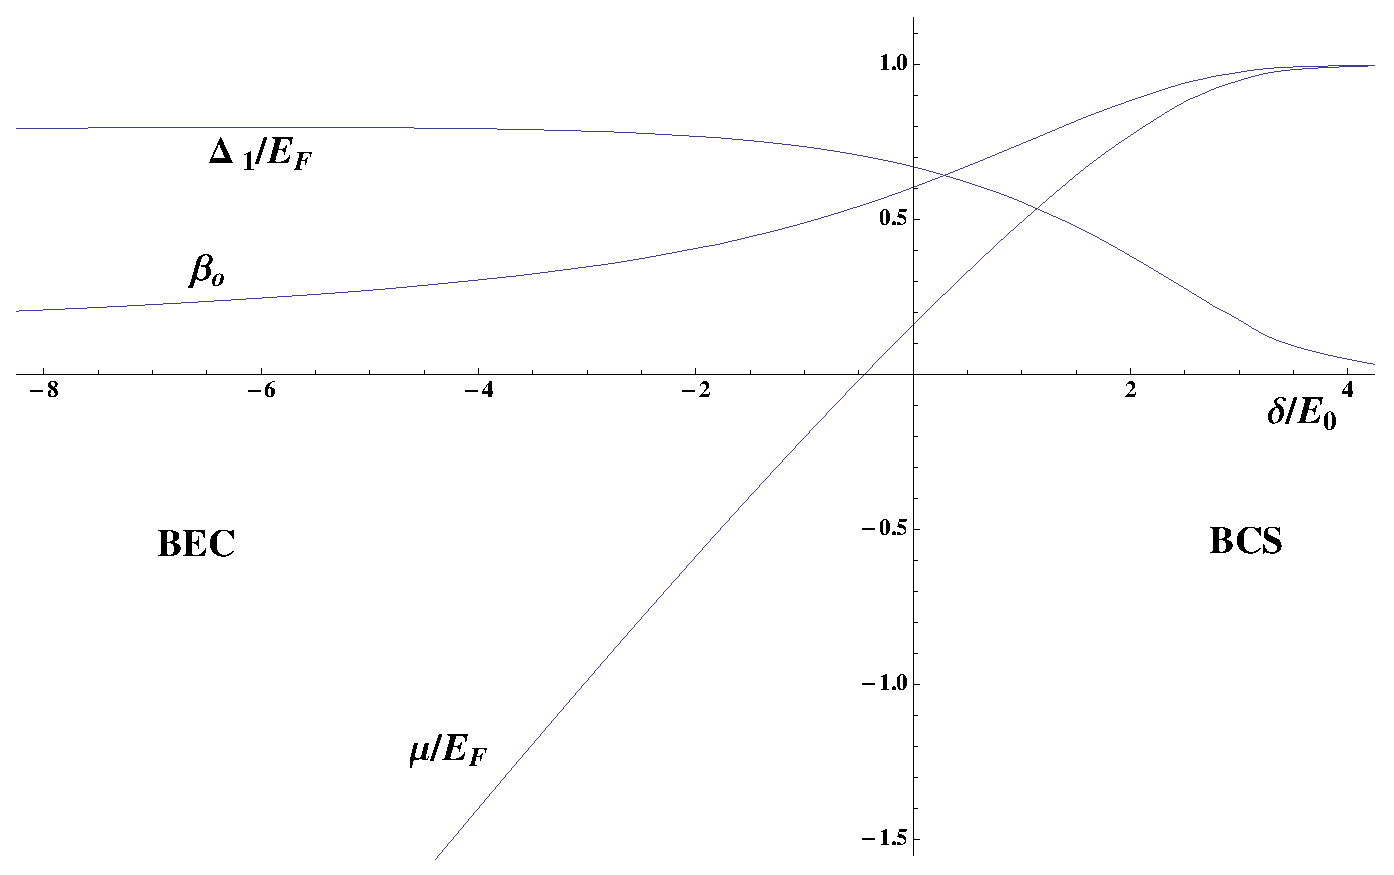
\includegraphics[width=0.8\textwidth]{narrow}
\caption{The chemical potential $\mu$, the open-channel gap $\Delta_{1}$ and the open-channel relative weight $\beta_{o}$ over crossover with the narrow Feshbach resonance without considering the inter-channel Pauli exclusion  vs. the chemical potential and the gap in the single-channel model} 
\label{fig:pathInt2:narrow}
{\small  The gap in the open-channel $\Delta_{1}$ and the chemical potential $\mu$ are rescaled with the the Fermi energy of the total density, $E_{F}^{(tot)}$.  The $x$-axis is the detuning $\delta$ rescaled with $E_{0}$ (see Eq. \ref{eq:pathInt2:E0}) for the narrow resonance; while it is $-1/a_{s}k_{F}$ for the single-channel curves. We have taken $\delta_{c}=0.001E_{F}^{(tot)}$ for the narrow resonance figure. We used the detuning from the resonant point  for the $x$-axis in the narrow resonance instead of $-1/a_{s}k_{F}$ in the single-channel because the additional shift, $2\mu$, considering in Eq. \ref{eq:pathInt2:simplenarrowAs}.  Consequently, the chemical potential lines in both cases cross the $x$-axis at the same point where $\mu=0$.  }
\end{center}
\end{figure}
}
\section[Excitation]{Excitation Mode}
\frame{
\frametitle{Fermionic modes and Bogoliubov transformation}
}
\frame{
\frametitle{Bosonic modes}
\begin{itemize}
\item Fluctuations of the order parameters;
\item Four possible modes for two complex order parameters ($\Delta_1$, $\Delta_2$);
\item The overall phase fluctuation mode is the Goldstone mode;
\item The other three modes are massive.

\end{itemize}
}